\documentclass[red]{beamer}


\mode<presentation> {
  \usetheme{Warsaw}
  \setbeamercovered{transparent}
}


\usepackage{beamerthemesplit} 
\usepackage[czech]{babel}
\usepackage[utf8]{inputenc}
\usepackage[T1]{fontenc}
\usepackage{listings}

\title{Distribuovaný systém kontroly verzií - Git}    
\author{Juraj Hreško}                 
\institute{ecommerce.cz}      
\date{\today}                 

\begin{document}

\begin{frame}
  \titlepage
\end{frame}


\section{Verzovacie systémy} % 1. Kapitola



\begin{frame}
  \frametitle{Požiadavky na SCM}   
  \begin{itemize}
  \item ukladanie dát do archívu (repozitára)

  \item obnovenie dát z určitej doby

  \item porovnávanie verzií dát

  \item anotovanie dát

  \item riešenie prítupu viacerých vývojárov

 \item označovanie verzií špecifickým menom

 \item vetvenie vývoja

 \item zlučovanie vetví vývoja
  \end{itemize}
\end{frame}

\begin{frame}
  \frametitle{Typy verzovacích systémov}   
  \begin{itemize}
  \item "triviálne"
  \item centralizované (client-server)
  \item distribuované
  \end{itemize}
\end{frame}

\begin{frame}[fragile]
  \frametitle{"Triviálne"  verzovanie}   
   
  Použil už snáď každý pri zálohe napr. konfiguračných súborov. 

\begin{block}{Príklad}
\begin{verbatim}
    $ cp config.cfg config.old
    c:\>copy config.cfg config.old
\end{verbatim}
\end{block}

\begin{itemize}
\item vhodné pre jednu dostupnú "zálohu"
\item nesystematické pre viac súborov s históriou
\item nehovoriac o zdieľaní, vetvení a pod.
\end{itemize}

\end{frame}

\begin{frame}
  \frametitle{Centralizované systémy pre správu verzií}   

\begin{itemize}
\item architektúra typu klient-server
\item spoločný centrálny repozitár
\item vývoj prebieha v rámci pracovnej kópie
\item riešenie súčasného zápisu viacerých programátorov
\begin{itemize}
\item lock/modify/commit
\item modify/merge/commit
 \end{itemize}
\item zástupcovia: CVS, SVN, Perforce, TFS
 \end{itemize}
\end{frame}

\begin{frame}
  \frametitle{Distribuované systémy pre správu verzií}   

\begin{itemize}
\item neexistuje centrálny repozitár - každý je plnohodnotný
\item miesto operácie checkout operácia clone
\item repozitár == pracovná kópia
\item publikovanie zmien - vystavenie repozitára, push do vzdialenej vetvy, posielanie záplat e-mailom
 \end{itemize}
\end{frame}

\section{Výhody DSCM (Git)} % 2. Kapitola

\begin{frame}
  \frametitle{Práca s lokálnym repozitárom}   

\begin{itemize}
\item neexistuje "jedno zraniteľné miesto" (single point of failure)
\item offline práca s repozitárom (vo vlaku, na chate, pri výpadku serverov)
\begin{itemize}
\item prechádzanie histórie
\item commity
\item vetvenie
 \end{itemize}
\item súkromie pri experimentoch
\item rýchlosť operácií
 \end{itemize}
\end{frame}

\begin{frame}
  \frametitle{Práca s repozitármi - schéma}

  \begin{figure}
  \centering
  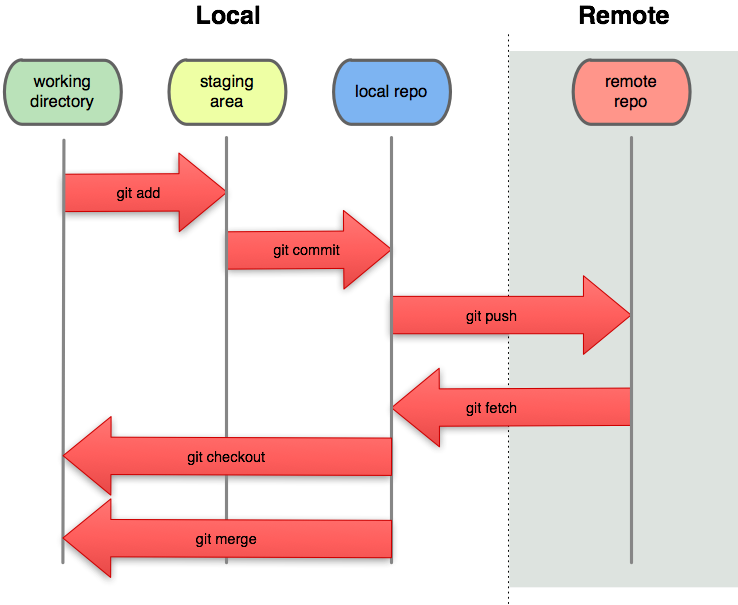
\includegraphics[scale=0.7]{git-pics/local-remote.png}
\end{figure}
\end{frame}

\subsection{Flexibilný workflow}
\begin{frame}
\frametitle{Flexibilný workflow}
\begin{itemize}
\item je možné pracovať s repozitármi rôznymi spôsobmi, v závislosti od druhu projektu
\item iné pre klasický centralizovaný vývoj, vlastné dokumenty, vývoj open source software
\item príklady niektorých možných workflow
\begin{itemize}
\item centralizovaný 
\item koordinátor
\item generál a pobočníci
 \end{itemize}
 \end{itemize}
\end{frame}

\begin{frame}
  \frametitle{Centralizovaný workflow}

  \begin{figure}
  \centering
  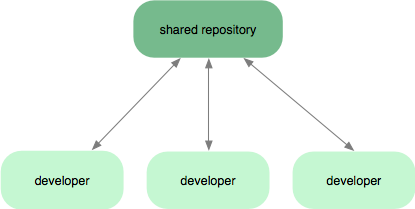
\includegraphics[scale=1]{git-pics/workflow-a.png}
\end{figure}
\end{frame}

\begin{frame}
  \frametitle{Workflow "koordinátor"}

  \begin{figure}
  \centering
  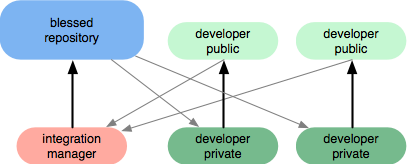
\includegraphics[scale=1]{git-pics/workflow-b.png}
\end{figure}
\end{frame}

\begin{frame}
  \frametitle{Workflow "generál a pobočníci"}

  \begin{figure}
  \centering
  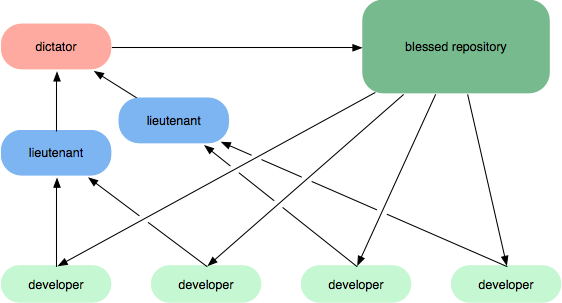
\includegraphics[scale=1]{git-pics/workflow-c.png}
\end{figure}
\end{frame}

\section{Git} % 3. Kapitola	

\subsection{Na úvod ku Gitu}
\begin{frame}
\frametitle{Krátko k histórii projektu}

\textbf{ git \\
 \textit{1.	a contemptible person, often a fool\\
2.	a bastard}} \\ 
\textbf{ \tiny{ (Collins English Dictionary)}}
\begin{itemize}
\item vznik v roku 2005, k účelu verzovania projektu linuxového jadra
\item hlavné požiadavky 
\begin{itemize}
\item Take CVS as an example of what not to do; if in doubt, make the exact opposite decision
\item Support a distributed, BitKeeper-like workflow
\item Very strong safeguards against corruption, either accidental or malicious
\item Very high performance
 \end{itemize}
\item spočiatku sada programov v Perl, Bash a C
 \end{itemize}
\end{frame}

\begin{frame}
  \frametitle{Súčasnosť projektu}   

\begin{itemize}
\item voľne dostupný open source DSCM software
\item stránky projektu \href{http://git-scm.com/}{http://git-scm.com/}
\item používaný aj na väčších projektoch
\begin{itemize}
\item Git
\item Linux Kernel
\item Android
\item Ruby on Rails
\item Fedora
\item VLC media player
\item \dots
 \end{itemize}
\item primárne pre platformu GNU/Linux a ostatné Unix-like systémy - BSD, Solaris, Darwin
\item pre MS Windows v Cygwin alebo port mysysgit
\item základom je ovládanie cez príkazový riadok, dostupné však aj GUI a pluginy pre IDE (Eclipse, NetBeans, Visual Studio)
 \end{itemize}
\end{frame}

\subsection{Práca s Gitom}

\begin{frame}[fragile]
\frametitle{Inštalácia}   

Pre GNU/Linux  balíček v repozitári - git-core
\begin{block}{Príklad}
\begin{verbatim}
$ yum install git-core		
$ apt-get install git-core		
\end{verbatim}
\end{block}
Pre MS Windows doporučujem kombináciu msysgit + TortoiseGit
\begin{itemize}
\item \href{http://code.google.com/p/msysgit/}{msysgit} - posledná verzia \href{ http://code.google.com/p/msysgit/downloads/detail?name=Git-1.7.2.3-preview20100911.exe}{Git 1.7.2.3}
\item pri výbere komponent doporučujem zrušiť Windows Explorer integration (zabezpečí ho TortoiseGit)
\item ostatné voľby podľa uváženia, osobne ponechávam východzie
\item následne doinštalovať GUI klienta - \href{ http://code.google.com/p/tortoisegit/}{TortoiseGit}
\item pri inštalácii je dobré zvoliť totožného SSH klienta ako u Gitu, v mojom prípade u oboch OpenSSH
 \end{itemize}
\end{frame}

\end{document}
